\chapter{Vergleich}
\label{ch:chapter05}
In diesem Kapitel werden die beiden Konzepte (Hierarchische Struktur und Minimalistisch) mittels eine Nutzwertanalyse betrachtet.
Diese sollen helfen zu betrachtet, welche der beiden Konzepte allgemein die vorher genannten Kriterien am meisten erfüllt.
Dabei werden die Ergebnisse der Prioritätsanalyse verwendet und basierend mit dem Erfolg, die das Konzept für das jeweilige Kriterium hat verrechnet und addiert.
Das Konzept mit einem höheren Wert erfüllt mehr die Kriterien als das andere.
Zum Abschluss wird die alternative racF begutachtet auf ihre Vor und Nachteile.

\section{ABC-Analyse}
\label{sec:chapter05:Anal}

\section{Nutzwertanalyse}
\label{sec:chapter05:Nutz}
Für die Nutzwertanalyse müssen die jeweiligen \ac{TN} bestimmt werden.
Dies wird mittels \ac{Gf} mal der \ac{Zf} gemacht.
Daraus bildet sich der \ac{TN} und die Summe davon generiert den \ac{GN}.
Der höhere \ac{GN} zeigt, dass dieses Konzept einen höheren Nutzen hat.
Anzumerken dabei ist, dass wenn die \ac{GN} zu ähnlich sind, weitere Schritte vorgenommen werden sollen, um ein eindeutiges Rank zu erschaffen.
Für die \ac{Zf} wurde wieder ein vier Punktesystem ausgewählt.
Die Tabelle (\ref{fig:Ziel}) zeigt was die verschiedenen Zahlen bedeuten. \cite{BdIufH}
\begin{figure}[h!]
 \centering
 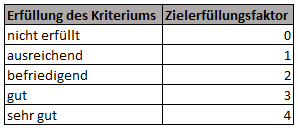
\includegraphics[width=1\textwidth]{gfx/Picture/Ziel.PNG}
 \caption{Die Zf Tabelle}
 \label{fig:Ziel}
\end{figure}
\newpage
\begin{figure}[h!]
 \centering
 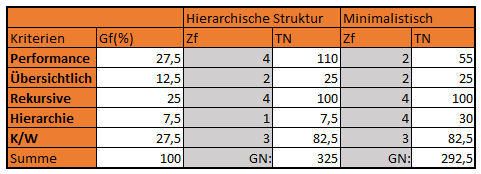
\includegraphics[width=1\textwidth]{gfx/Picture/Nutzwert.PNG}
 \caption{Nutzwertanalyse für die beiden Konzepte}
 \label{fig:Nutz}
\end{figure}

Wie man erkennen kann ist der \ac{GN} zwischen den beiden Faktoren bei $70$.
Da kein Unterschied erkannt werden kann, wird die Wermaßstäbe weiter verfeinert.
Dadurch ändert sich die Punkteskala und Tabelle wie folgt:
\begin{figure}[h!]
 \centering
 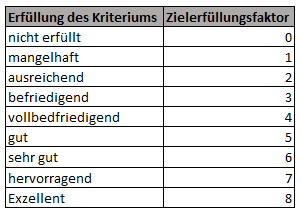
\includegraphics[width=1\textwidth]{gfx/Picture/Ziel2.PNG}
 \caption{Die Zf Tabelle}
 \label{fig:Ziel}
\end{figure}
\newpage
\begin{figure}[h!]
 \centering
 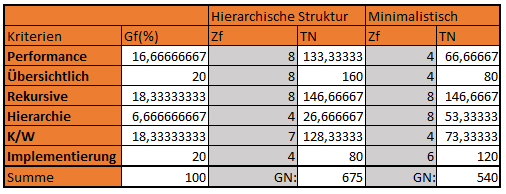
\includegraphics[width=1\textwidth]{gfx/Picture/Nutzwert2.PNG}
 \caption{Nutzwertanalyse für die beiden Konzepte}
 \label{fig:Nutz}
\end{figure}
Durch die Verfeinerung liegt der Unterschied zwischen den beiden Faktoren bei $135$.
Wodurch das Konzept Hierarchische Struktur eindeutig im Rank an erste Stelle steht.

\section{Vor/Nachteile Hierarchische Struktur}
\label{sec:chapter05:Hierarchische}
Bei der ersten Tabelle (\ref{fig:Ziel}) wurde der Hierarchische Struktur für Performance vier, Übersichtlich vier, Rekursive vier, Hierarchie eins, \ac{K/W} vier und Implementierung zwei Punkte gegeben.
Die Performance hat vier bekommen, da die Effizienz durch den Algorithmus im Allgemeinfall um die 50 mal effektiver ist.
Dies ist eine enorme Steigerung weshalb es die maximale Punktzahl bekommen hat.
Übersichtlich hat vier Punkte erhalten, weil die Entwickler einstimmig dieses Konzept als übersichtlicher empfinden.
Zudem ist es einfach festzustellen, welches Profil, welche Aufgabe hat.
Aber es hat zwei Punkte verloren dadurch, dass die Graphik bei weiteren Profilen schwieriger zu lesen wird, da diese groß ist.
Rekursive hat vier Punkte erlangt, da es durch die Regelung, dass Profile nur noch Profile oder Berechtigungen enthalten sowie die feste Struktur keine Rekursivenbeziehungen möglich sind, sofern man nicht aktive gegen die Regelungen verstößt.
Deshalb hat es wie Performance vier Punkte erhalten.
Für die Hierarchie hat die Struktur nur einen Punkt bekommen, weil es bei diesem Punkt darum ging die Hierarchie so stark wie möglich zu verringern.
Es ist besser als die vorherige Hierarchie, aber ist dennoch sehr hierarchisch.
Die \ac{K/W} haben nur vier Punkte bekommen, da nach der Entwicklung der Profile, diese nicht mehr geändert werden sollen.
Die Implementierung hat lediglich zwei Punkte bekommen, da diese aufwendig.
\newline
\newline
Nachdem die \ac{Zf} erweitert wurde, haben sich die Werte wie folgt verändert.
Die Performance wurde acht Punkte, Übersichtlich acht, Rekursive acht, Hierarchie vier, \ac{K/W} sieben und Implementierung vier Punkte gegeben.
Wie schon im vorherigen Absatz angegeben kann dieses Konzept 50 mal effektiver sein.
Deshalb habe diesem Punkt exzellent gegeben, da dies eine deutliche Verbesserung ist.
Übersichtlich hat eine exzellelte Bewertung erhalten.
Die Struktur ist geordnet nach den Fachbereichen und hat ein hierarchie Limit von vier.
Dies ist der Rahmen wodurch die IT-Spezialisten dies als übersichtlich befinden.
In der Kategorie Rekrusive ändert sich nicht viel, weshalb es wieder volle Punktzahl erlangt.
Hierarchie hat vier Punkte bekommen, da die hierarchie wenn auch nur minimal verringert wurde.
Dies würde nur drei Punkte geben, aber da es auch die hierarchie Stufe auf vier limitiert wurde dies einen weiteren Punkt gegeben.
\ac{K/W} hat nur sieben statt acht Punkte bekommen, da dieses Konzept, trotz dessen, dass es nicht geändert werden soll, in einem regelmäßigen Zyklus gewartet werden muss.
Dies liegt daran, dass man überprüfen muss, ob nicht ein Entwickler aus Faulheit die Struktur geändert hat.
Daher ist es eine hervorragende Lösung, aber man muss dennoch etwas berücksichtigen.
\newline
\newline
Zusammenfassend hat das Konzept Hierarchische Struktur viele positive Aspekte.
Unter diese Fallen zum Beispiel die erhöhte Performance sowie Rekursive und Übersichlichkeit.
Auf der anderen Seite ist dieses Konzept weiterhin sehr hierarchisch sowie ist die Implementierung aufwendig.
Dies würde einiges an personen Tagen sowie weiteres Geld kosten.

\section{Vor/Nachteile Minimalistisch}
\label{sec:chapter05:Minimalistisch}
Das Minimalistisch Konzept hat für Performance zwei, Übersichtlich eins, Rekursive vier, Hierarchie vier, \ac{K/W} zwei und Implementierung vier Punkte erhalten.
Durch die verringerte Struktur hat sich die Performance ebenso verbessert, aber dies ist keine permanente Lösung, da ein Steigen von Profilen diesen Bonus nichtig macht.
Aus diesem Grund hat es nur zwei Punkte bekommen.
Übersichtlich hat es nur einen Punkte erlangt.
Auch wenn durch das entfernen der Hierarchie weniger Verwirrung herrscht, ist es dennoch sehr unübersichtlich, wenn alle Berechtigungen mit Außnahme der standard Berechtigunen, direkt am Profil hängen.
Da es keine tiefe Hierarchie mehr gibt, ist es auch unmöglich, dass es eine Rekursion gibt.
Weshalb dieses Konzept in diesem Punkt die maximale Anzahl von Punkten erlangt.
Wie schon angesprochen geht es bei dem Punkt Hierarchie darum die Hierarchie so stark wie möglich zu reduzieren und dieses Konzept hat die Hierarchiestruktur auf ein Minimum gebracht und erhält daher vier Punkte.
Die \ac{K/W} haben zwei Punkte erlangt, da diese regelmäßig überprüft werden müssen, dass Entwickler nicht aus verschiedenen Gründen zusätzliche Profile hinzufügen.
Dies ist eine Sorge, da genau dies zur unübersichtlichen Berechtigungsstruktur gesorgt hat, die die Helvetia aktuell hat.
\newline
\newline
Nach der Spezifizierung hat sich die Bewertung von das Minimalistisch Konzept wie folgt geändert.
Die Performance wurde vier Punkte, Übersichtlich vier, Rekursive acht, Hierarchie acht, \ac{K/W} vier und Implementierung sechs Punkte gegeben.
Der Punkt Performance hat befriedigend bekommen, vier die neue Struktur diese eine Verbesserung ist, aber dies sich ändern kann.
Übersichtlich hat gut statt ein vollbefriedigend erhalten, weil selbst wenn es auch schwieriger ist übersichtlich zu sehen, welche Berechtigungen alle einem Profil zu geordnet wurden, ist es dennoch leichter herauszufinden, wer alles eine spezifische Berechtigungen hat.
Dies liegt daran, dass die Berechtigungen nicht mehrmals an verschiedenen Stellen dem Profil zu gewissen werden.
Rekursive erlangt ein exzellent, da es nicht möglich ist eine rekursive Beziehung zu erstellen bis auf, wenn ein Standardprofil auf sich selber zeigt.
Hierarchie ebenso wie Rekursive bekommt ein exzellent, da eine weitere reduktion der Hierarchie für lediglich mehr Chaos sorgen würde, da dann alle Berechtigungen direkt am Nutzer hängen würden.
\ac{K/W} erlangt eine vier. 
Das Minimalistisch Konzept hat nicht viele Konvention, die überprüft werden müssen sowie ist die Überprüfung einfach, da die Struktur so minimalistisch ist, aber es regelmäßig überprüft werden muss und das Risiko, dass ein Entwickler die Struktur ändert ist hoch.
\newline
\newline
Zusammenfassend kann gesagt werden, dass das Minimalistisch Konzept am Hilfsreichsten ist, wenn man nach spezifischen Berechtigungen sucht.
Durch die minimale Hierarchie gibt es nicht viele Stellen, die überprüft werden müssen sowie Stellen an denen Rekursionen entstehen können.
Auf der anderen Seite ist jedoch die Verbesserung der Performance ist nicht stabile und kann sich schnell ändern, wenn weitere Profile hinzugefügt werden.
Die Implementierung ist im Verhältnis zum Hierarchische Struktur Konzept deutlich einfacher, da für jeden Fachbereich die Standardprofil entwickelt werden müssen und ansonsten die restlichen Berechtigungen direkt an die Nutzer zu geteilt werden und keine neuen Profile entwickelt werden müssen.
Jedoch besteht die Gefahr, dass bei der Menge von Berechtigungen gewisse Nutzer bestehende verlieren.

\section{Ablösung ins racF}
\label{sec:chapter05:racF}
Donec gravida consequat arcu, et mollis tortor posuere vitae. Sed pharetra turpis a ante commodo accumsan. Suspendisse leo nulla, accumsan sit amet dapibus in, posuere eget turpis. Vivamus enim sapien, porta id placerat eget, laoreet sed massa. Class aptent taciti sociosqu ad litora torquent per conubia nostra, per inceptos himenaeos.

